\documentclass[11pt]{article}
\usepackage[margin=1in]{geometry}
\usepackage{enumitem}
\usepackage{booktabs}
\usepackage{xcolor}
\definecolor{cieblue}{RGB}{31, 119, 180}
\usepackage[colorlinks=true]{hyperref}
\hypersetup{
    linkcolor=cieblue
}
\usepackage{amsmath,amssymb}
\usepackage{graphicx}
\usepackage{float}
\usepackage{tocloft}
\setlength{\cftbeforesecskip}{3pt}
\setlength{\cftbeforesubsecskip}{1pt}
\renewcommand{\cftsecfont}{\bfseries}
\renewcommand{\cftsecpagefont}{\bfseries}
\renewcommand{\cftsecleader}{\cftdotfill{\cftdotsep}}
\renewcommand{\thefootnote}{\textcolor{red}{\arabic{footnote}}}

\setlength{\parskip}{6pt}
\setlength{\parindent}{0pt}

\title{Optimization-Based Decision Support for Equitable Expansion of\\
Federally Qualified Health Centers in Chicago}

\author{Alaittin Kirtisoglu\thanks{Department of Applied Mathematics,
Illinois Institute of Technology, Chicago, IL 60616.
E-mail: \texttt{akirtisoglu@hawk.iit.edu}} \and
Hemanshu Kaul\thanks{Department of Applied Mathematics,
Illinois Institute of Technology, Chicago, IL 60616.
E-mail: \texttt{kaul@iit.edu}}}

\date{March 2026}

\begin{document}

\maketitle

\begin{abstract}
\noindent This report presents a spatial optimization framework for equitable expansion of Federally Qualified 
Health Centers in Chicago. We document four critical gaps in the current system: the absence of location evaluation 
tools for decision-makers, an obsolete Index of Medical Underservice (IMU) formula, a limited MUA designation process, and 
unmapped referral networks despite federal mandates. We describe how optimization can address each 
one. We report on the data infrastructure and the interactive dashboard we have been developing, and outline what 
our optimization model can deliver: design of catchment areas and larger health zones, facility location analysis, and redesigned 
IMU formulas. The report includes a roadmap for the next steps.
\end{abstract}

\vspace{6pt}
\tableofcontents
\newpage

\section{The Problem and Motivation}\label{sec:problem}

Chicago's primary care safety net is operated largely through Federally Qualified Health Centers (FQHCs), 
community-based clinics that receive federal funding through HRSA's Health Center Program to serve low-income 
and uninsured populations regardless of ability to pay. In Chicago, 25 parent organizations operate 166 primary 
care FQHC sites (obtained from 213 total sites by removing shelters, school-based outreach, and administrative 
offices), managed under 1,363 grants awarded by HRSA's Bureau of Primary Health Care between 2016 and 
2026~\cite{hrsa2026data}. Nationally, in 2024 more than 32.4 million people used HRSA-funded health centers 
through 139.4 million total visits; about 90\% of these patients had incomes at or below 200\% of the federal 
poverty level, including 25.1 million uninsured, Medicaid, and Medicare patients~\cite{hrsa2026data}. Federal 
appropriations have grown from \$554 million in 1990 to over \$6 billion today~\cite{crs2017healthcenters}. 
Since 2014, the number of medically underserved people has nearly doubled from 56 million to over 100 million; 
a study commissioned by NACHC found that over 100 million people in the United States may not have access
to a usual source of primary care due to a shortage of providers in their
community~\cite{NACHC2014}. 

HRSA regulates FQHCs through the Health Center
Program Compliance Manual~\cite{bphc2025compliance},
which imposes requirements that are spatial
planning problems:

\begin{enumerate}[nosep, label=\textbf{R\arabic*.}]
    \item \label{r:catchment} \textbf{Catchment area design} (Ch.~3): Health centers must define and annually 
    review the boundaries of the catchment area to be served such that the area's size ensures services are 
    available and accessible to the residents of the area promptly; boundaries must eliminate, to the extent 
    possible, barriers resulting from the area's physical characteristics, its residential patterns, its economic 
    and social groupings, and available transportation.
    \item \label{r:needs} \textbf{Needs assessment} (Ch.~3): Centers must assess unmet need using available health 
    resources in relation to the size of the area and its population, including appropriate ratios of primary care 
    physicians, along with health indices (infant mortality), economic factors (poverty rate), and demographic 
    factors (population 65+), the exact four components of the IMU score.
    \item \label{r:locations} \textbf{Accessible locations} (Ch.~6): Sites must be accessible to the patient population 
    relative to where this population lives or works, considering access barriers and distance and time taken 
    for patients to travel to or between service sites.
    \item \label{r:referral} \textbf{Hospital referral relationships} (Ch.~8): Each center must develop an ongoing 
    referral relationship with one or more hospitals to assure continuity of care within the catchment area.
    \item \label{r:collaborative} \textbf{Collaborative relationships} (Ch.~14): Centers must establish and maintain 
    collaborative relationships with other health care providers within the catchment area, local hospitals, and 
    specialty providers to reduce the non-urgent use of hospital emergency departments.
\end{enumerate}

Each of these requirements involves spatial decisions such as where to draw boundaries, how to measure accessibility, 
which hospitals to partner with, yet HRSA provides no quantitative tools for making them. Health centers are left to 
determine these on their own, and the results are uneven. Below we identify four
critical gaps in the current system.

\medskip

\label{gap:location}\textbf{Gap 1: Decision makers have no way to evaluate a location.} When an organization applies for an 
HRSA New Access Point grant, it must justify \emph{why this location}. But there is no tool to answer that 
question rigorously. How many underserved residents are within 30 minutes by transit? What is the current 
capacity of nearby facilities? Will the new site relieve overloaded neighbors or duplicate existing coverage? 
Nationally, Chang et al.~\cite{chang2019geographic} showed that new FQHCs certified between 2007 and 2014 
were much less likely to be in high-poverty areas than existing ones (20.5\% vs 31.4\%). Lee et al.~\cite{lee2023spatial} found that
FQHC patient volume is 3.27 times higher in areas
with at least one FQHC than in areas with none,
confirming that spatial availability directly drives
utilization. Despite a large body of work on healthcare facility
location models, no published study has applied
spatial optimization specifically to FQHC site
selection. The current system responds to where
grant applications originate, not where need is
greatest.

\medskip

\label{gap:imu}\textbf{Gap 2: The IMU score is outdated.} HRSA designates Medically Underserved Areas (MUAs) using the 
Index of Medical Underservice (IMU), a composite of four indicators: provider-to-population ratio, infant 
mortality, poverty rate, and percentage aged 65+. Each is converted to a 0 to 25 scale and summed. The 
total IMU score ranges from 0 to 100, where lower values indicate greater underservice. Areas scoring IMU 
$\leq$ 62 qualify as medically underserved. But this formula dates from the 1970s. Ricketts et 
al.~\cite{ricketts2007designating} argued nearly 20 years ago that the method no longer captures 
modern healthcare access barriers. It omits insurance coverage, a primary barrier to care. It omits 
transportation access, often the main factor in
whether a clinic is reachable. It omits chronic 
disease burden (diabetes, hypertension, obesity), the conditions FQHCs actually treat. And it uses a hard 
binary cutoff: two neighboring tracts with IMU scores 63 and 62 are considered not eligible and eligible, 
respectively. Moreover, a tract scoring 61 and a tract scoring 30 are treated identically, even though their 
needs are vastly different. Ricketts et
al.~\cite{ricketts2007designating} also proposed a
data-driven replacement, and HRSA issued a Federal
Register proposed rule in 2008 to adopt it, but the
rule was never finalized. No alternative scoring
system has been developed at the research level
since.

\medskip

\label{gap:mua}\textbf{Gap 3: The MUA designation process has significant limitations.} To obtain an MUA designation, 
an organization must submit an application to HRSA proposing a rational service area, typically a 
group of census tracts. The applicant draws the boundary, not HRSA~\cite{bphc2025compliance}. HRSA then 
computes the IMU score for the proposed area. This means boundaries can be \emph{manipulated} to push 
IMU below 62, there is no systematic process to determine which groupings of tracts \emph{should} be 
designated, and communities without an organization capable of navigating the federal application never 
get designated at all. Ricketts et al.~\cite{ricketts2007designating} argue that this applicant-driven 
process systematically excludes communities that lack an organization capable of navigating the federal 
designation system. Milano~\cite{milano2025spatial} found a similar pattern statewide in New Jersey: 1,139 
census tracts scored medium or high risk on a composite access index, but only 248 held MUA designation. 
In Chicago, Kim et al.~\cite{kim2020uneven} found that 87 census tracts meet IMU eligibility but lack formal 
designation, predominantly on the South Side. Between 2009 and 2012, 12 clinics closed while 68 opened, yet 
MUA-eligible but undesignated tracts received only 3 new FQHCs compared with 41 in designated tracts. The 
resulting FQHC rate in undesignated tracts was only 15.5 per 100,000 poor, versus 40.8 in designated areas. 
The designation gap is built into the process.

\medskip

\label{gap:referral}\textbf{Gap 4: HRSA requires referral agreements but provides no network analysis.} Ch.~8 requires that each health 
center develop an ongoing referral relationship with one or more hospitals. Ch.~14 requires collaborative relationships 
with local hospitals and specialty providers to reduce the non-urgent use of hospital emergency departments. But which 
hospital should a given clinic partner with? Are there communities where patients have no viable referral path to specialist 
care? Research shows only 34.8\% of referrals in the U.S. result in completed specialist visits \cite{patel2018closing}, 
and the failure rate is worse in underserved areas. No city-level physician referral network has been
constructed for Chicago or any other US city, existing
work~\cite{an2018analysis} operates only at the
national level.

\medskip

These gaps are connected. In 2005, the Chicago
Department of Public
Health~\cite{salem2005casting} documented that the
ratio of safety net capacity to medically needy
population varied tenfold across regions,
from 0.4 in the Northwest to 5.1 in the Central
region. There were 484,120 low-income uninsured
Chicagoans, and only 35\% received community-based
care; 312,395 had no medical home. The South region saw visits decline even as
the number of sites
increased, suggesting that \emph{where} facilities
are placed matters as much as \emph{how many}. Two
decades later, HRSA still tracks grants at the
organization level, not the site level, with no
public tools to evaluate whether funding reaches
the neighborhoods with the greatest need.
P\'{e}rez et al.~\cite{perez2021decision} found
through optimization modeling that more funding does
not always lead to better health outcomes: more
sites do not help if they are in the wrong places.

People in poor, predominantly Black neighborhoods
on Chicago's South Side have a life expectancy 30
years shorter than those in wealthy neighborhoods
nine miles away, the largest such gap in the United
States~\cite{smithcommunity}. Luo et
al.~\cite{luo2022spatial} showed on the same South
Side that better spatial accessibility to primary
care is associated with lower hypertension
prevalence. Lee et al.~\cite{lee2023spatial} studied
six states including Illinois and found that in MUAs
with at least one FQHC, patient volume was 3.27 times
higher than in MUAs with none, and that FQHC placement patterns may
reflect historic redlining.\footnote{Redlining was a federal housing
policy from the 1930s where the Home Owners' Loan
Corporation (HOLC) graded neighborhoods A through D.
Banks refused loans in those areas for decades. The
same neighborhoods received less investment in
infrastructure, healthcare, schools, and housing
for generations. Lee et al.~\cite{lee2023spatial}
found that FQHC placement patterns today still
correlate with these historical grades, meaning
formerly redlined neighborhoods remain underserved.}
These patterns suggest a long-standing
mismatch between where facilities are placed and
where they are most needed.

In summary, \hyperref[gap:location]{Gap~1} is
addressed by the district and superdistrict design
in Section~\ref{sec:approach}, which lets decision makers evaluate candidate locations against existing capacity, demand, and a user-defined IMU-like score. \hyperref[gap:imu]{Gaps~2} and~\hyperref[gap:mua]{3} are addressed by the redesigned IMU-like scores in
Section~\ref{sec:imu}. \hyperref[gap:referral]{Gap~4} is
addressed at the superdistrict level through
hospital referral relationships, and more fully in the follow-up study proposed in
Section~\ref{sec:future}.


\section{Model Formulation}\label{sec:model}

The problems described above involve making spatial decisions under constraints such as budget, 
capacity, travel time, equity, with many interacting components. We propose a spatial 
optimization framework that addresses the HRSA
requirements listed in Section~\ref{sec:problem}.


\subsection{A hierarchical network design via FalCom}

Geographic disparities in healthcare access have been studied across multiple service domains. In organ allocation, Gentry et al.~\cite{gentry2015gerrymandering} used integer programming to redistrict U.S.\ liver allocation regions for equity, and Akshat et al.~\cite{akshat2024heterogeneous} extended this with heterogeneous donor circles that equalize supply-to-demand ratios under contiguity and capacity constraints. The HRSA/FQHC setting we study shares the same structural form: supply and demand on a fixed geographic graph with capacity, contiguity, and equity constraints, where boundary design is itself a policy lever.

FalCom~\cite{kirtisoglu2026falcom} is a Markov chain Monte Carlo
method designed for hierarchical and capacitated facility location
and districting problems. The energy of a district measures how well a facility
within that district serves its demand points. The system can be designed in a way that energies (service qualities) across districts are equalized.
The sampler favors configurations where no district is
left with disproportionately high energy. The energy function is user-defined and can serve as
an access measure, incorporating any combination of
factors such as population-provider ratio, travel time,
insurance coverage, or chronic disease burden. Given a set of facilities, demand units, and an energy 
function, FalCom generates a collection of high-quality spatial 
configurations, each assigning demand units to facilities and grouping
facilities into higher-level health zones, rather than returning a single 
optimal solution. This allows decision makers to compare alternative 
configurations and choose locations based on their priorities. The model organizes 
Chicago's healthcare landscape into two levels, matching the structure HRSA requires:


\textbf{Districts} are the catchment areas for primary care that HRSA's \textbf{R1} (catchment area design) requires 
each health center to define. Each district groups a set of census tracts around one FQHC or clinic. Today, health centers draw these 
boundaries case-by-case, without a formal methodology. Our model draws them systematically. We construct boundaries so that:
\begin{itemize}[itemsep=1mm]
    \item \textbf{Catchment area design.} District boundaries are geographically contiguous and respect residential patterns, 
    economic groupings, and available transportation, satisfying the Catchment Area Design requirement \textbf{R1} in the 
    Compliance Manual. The model determines a high-quality grouping of census
    tracts into catchment areas.
    \item \textbf{Needs assessment.} Each district maintains demand-capacity balance, i.e., the ratio of patients to
    available provider capacity is properly adjusted, satisfying the Needs Assessment requirement \textbf{R2} in the Compliance
    Manual. The district's energy value corresponds to its IMU score, linking the optimization directly to HRSA's underservice metric.
    \item \textbf{Accessible locations.} Every resident is assigned to a facility based on an access function $\mathrm{Access}(x, y)$,
     where $x$ is a facility and $y$ is a demand unit. The framework supports any definition of access (e.g., travel time, distance, 
     provider availability, or a composite), and we consider travel times via the CTA transportation network. For any such definition, the 
     model constructs rounded and equitable districts in terms of access, satisfying the Accessible Locations requirement \textbf{R3} 
     in the Compliance Manual.
\end{itemize}

\textbf{Superdistricts} group multiple primary care districts around a referral hospital. Each superdistrict ensures that every 
clinic within its boundaries has a clear referral path to a hospital and specialist care. Superdistricts are designed so that:
\begin{itemize}[itemsep=1mm]
    \item \textbf{Hospital referral relationships.} Each primary care site is linked to a hospital its patients can reach, 
    satisfying the Hospital Referral Relationships requirement \textbf{R4} in the Compliance Manual. The superdistrict 
    energy measures referral connectivity, i.e., how well patient flows stay within the superdistrict for specialist care.
    \item \textbf{Collaborative relationships.} Clinics within a superdistrict share a referral hub, strengthening the
    Collaborative Relationships requirement \textbf{R5} in the Compliance Manual and reducing fragmented care and non-urgent
    emergency department use. Fishman et al.~\cite{fishman2018spatial} found that in Chicago, patients in areas with lower
    spatial access to primary care had significantly higher odds of preventable emergency department use.
\end{itemize}

The framework uses CTA public transit travel times rather than straight-line distance as the access metric, directly addressing the requirement in Ch.~6. In Chicago, 36.9\% of African American households lack a vehicle~\cite{ermagun2020equity}; Ermagun and Tilahun showed that 50\% of African Americans in Chicago live in the lowest third of transit accessibility areas, compared to 21\% of whites. Milano~\cite{milano2025spatial} found that only 8\% of at-risk populations in New Jersey could reach an FQHC within 15 minutes by bus, regardless of time of day. A clinic 2 miles away may require a 45-minute bus trip. Using the actual transit network ensures that \emph{close} means close for the people who need the care. Balance can also be enforced across superdistricts, for example ensuring no superdistrict carries a disproportionately high uninsured rate or chronic disease burden.


\subsection{Continuous IMU Scoring}\label{sec:imu}

HRSA designates Medically Underserved Areas using the Index of Medical Underservice (IMU), a composite of four indicators converted to a 0--100 scale, with areas scoring $\leq 62$ qualifying as underserved (\hyperref[gap:imu]{Gap~2}). The formula dates from the 1970s and has structural problems: conversion tables are calibrated to 1970s national distributions; the linear sum cannot capture compounding disadvantage; the $0$--$25$ mapping compresses differences at the extremes; and a hard threshold treats two tracts scoring 62 and 63 as categorically different while treating tracts at 61 and 30 as identical.

Beyond these arithmetic problems, Ricketts et al.~\cite{ricketts2007designating} proposed a data-driven replacement with regression-derived weights. HRSA adopted it in a 2008 proposed rule~\cite{HRSA2008proposed} but withdrew it after negative public comments. A 1998 attempt met the same fate, and a 2010 ACA-mandated rulemaking committee voted 21--2 in favor without HRSA acting. Every attempt has failed because the IMU is fused to a binary funding decision tied to Section~330 of the Public Health Service Act, the statute that authorizes HRSA's Health Center Program grants to FQHCs~\cite{crs2017healthcenters}:
\[
\text{IMU} \leq 62 \;\implies\; \text{MUA designation} \;\implies\; \text{Section~330 funding eligibility.}
\]
Losing MUA status means losing federal grants, enhanced Medicare/Medicaid reimbursement, NHSC loan repayment placements, and J-1 visa waivers for international physicians. A new formula may show an area is no longer underserved on paper, but the facility there exists only because of the designation funding. The cutoff also creates a \emph{dilution problem} with honest boundary design: a district spanning a high-need and a moderate tract may average to IMU~63, even though half its population is severely underserved (\hyperref[gap:mua]{Gap~3}). Kim et al.~\cite{kim2020uneven} found 87 individually eligible but undesignated tracts in Chicago; grouping them into contiguous districts would average some above the threshold.

There is a deeper problem with the threshold. The IMU measures poverty, infant mortality, elderly share, and provider supply. FQHC funding does not reduce poverty or infant mortality; it provides healthcare access. An area that receives an FQHC will still be poor, still have high infant mortality, still have an aging population. The IMU barely changes whether a site is funded or not. The threshold tests for a condition that persists regardless of the intervention. The right question is which areas are worst off relative to others, and to fund those first, even if every district in the city scores above 62.

\medskip

\noindent\textbf{Continuous need score.} We replace the binary cutoff with a percentile-rank construction. Let $\mathcal{T}$ denote the set of all Chicago census tracts with $|\mathcal{T}| = N$, and let $x_k(t)$ denote the value of indicator $k$ at tract $t \in \mathcal{T}$ (Table~\ref{tab:indicators}). Each indicator is oriented so that higher values correspond to greater need (e.g., higher poverty rate, higher uninsured rate, higher infant mortality). The rank of $t$ on indicator $k$ is
\begin{equation}\label{eq:rank}
  \mathrm{rank}_k(t) \;=\; \bigl|\{t' \in \mathcal{T} : x_k(t') \leq x_k(t)\}\bigr|,
\end{equation}
the number of tracts whose indicator-$k$ value is at most that of $t$. The percentile rank is
\begin{equation}\label{eq:score}
  \varphi_k(t) \;=\; \frac{\mathrm{rank}_k(t)}{N} \;\in\; [0, 1].
\end{equation}
A tract at the 85th percentile on poverty scores $\varphi_k(t) = 0.85$. The overall need score averages across $K$ indicators:
\begin{equation}\label{eq:need}
  S(t) \;=\; \frac{1}{K} \sum_{k=1}^{K} \varphi_k(t) \;\in\; [0,1].
\end{equation}
This is the percentile-rank construction used by the CDC Social Vulnerability Index~\cite{CDC_SVI}. It is robust to outliers, requires no parameter tuning, and produces a continuous measure where higher values mean greater need. User-adjustable weights $w_k$ in place of $1/K$ allow decision makers to specify which factors matter most.

\begin{table}[H]
\centering
\caption{Indicators for the continuous need score.}
\label{tab:indicators}
\begin{tabular}{llll}
\toprule
\textbf{Category} & \textbf{Indicator} & \textbf{Source} & \textbf{Level} \\
\midrule
Access   & Provider-to-population ratio          & NPPES+Census & Tract  \\
Access   & Transit time to nearest provider      & CTA GTFS + OSM & Block \\
Coverage & Uninsured rate                        & Chicago Health Atlas & Comm.\ area \\
Burden   & Diabetes prevalence                   & Chicago Health Atlas & Comm.\ area \\
Burden   & Hypertension prevalence               & Chicago Health Atlas & Comm.\ area \\
Demog.   & Poverty rate                          & ACS 5-Year  & Tract  \\
Demog.   & \% aged 65+                           & Decennial   & Block  \\
Demog.   & Infant mortality rate                 & Chicago Health Atlas & Comm.\ area \\
\bottomrule
\end{tabular}
\end{table}

The indicators in Table~\ref{tab:indicators} combine fixed population characteristics (poverty, age structure, infant mortality) with access conditions that depend on where facilities sit (provider-to-population ratio, transit time to the nearest provider). We use the need score $S(t)$ directly as FalCom's district energy. FalCom chooses facility locations; each tract is assigned to the facility serving it, and the resulting catchment is the district. A district's energy is the population-weighted average of $S(t)$ over its tracts, and the sampler favors location configurations that equalize this score across districts. Demand--capacity balance is enforced as a separate per-district constraint within FalCom rather than baked into the indicator list.

\medskip

\noindent\textbf{Extensions.} Three further directions extend the basic continuous score:

\begin{enumerate}[nosep]
    \item \textbf{Probabilistic IMU.} Two of the four classical IMU indicators carry substantial uncertainty. Poverty rate and proportion aged 65+ come from the American Community Survey, where in approximately 50\% of census tracts the margin of error exceeds 50\% of the estimate itself~\cite{spielman2014patterns}. Instead of a single deterministic score, we can model each indicator with its uncertainty distribution and produce a \emph{probability of being underserved} for each tract. A tract with point-estimate IMU~63 but high variance might have a 40\% probability of actually falling below 62. This naturally handles measurement error.

    \item \textbf{Census block-level projection.} The current system computes IMU at the census tract or higher levels, masking within-area variation. We can project indicators down to census-block level using 2020 Decennial Census block data (population, age 65+) and ACS tract-level estimates (poverty, provider counts). This reveals where sharp cutoffs actually fall: a tract scoring 63 (not designated) may contain blocks that are severely underserved but invisible to the current system.

    \item \textbf{User-configurable indicator set.} The base score already extends beyond the four classical IMU indicators (Table~\ref{tab:indicators}), and the framework accepts any further indicators the data supports (e.g., language access, food insecurity, mental-health burden, housing instability), with user-adjustable weights. Rather than proposing a single replacement formula, this separates the policy question (what should count as underserved?) from the technical question (given a definition, where should facilities go?).
\end{enumerate}


\subsection{Patient Flow Model}\label{sec:flow}

Given a facility configuration produced by FalCom, the patient flow model assigns patients from tracts to facilities and returns the per-district demand--capacity check that the sampler uses to accept or reject the configuration. The supply side comes directly from data: HRSA's Uniform Data System (UDS) reports visits $v_j$ at each existing facility, and workforce FTEs combined with a visits-per-FTE benchmark give facility capacity $c_j$. Travel cost $t_{ij}$ is the CTA public transit time from tract $i$ to facility $j$.

Tract-level demand $d_i$ is the one quantity not directly observed, since UDS records visits at the destination rather than at the origin. We model
\[
  d_i = \rho_i \cdot D_i^\star,
\]
where $D_i^\star$ is a latent potential demand set by tract population and the need score $S(t_i)$, and $\rho_i \in [0,1]$ is a realization rate that rises with access to a nearby facility. The rate is calibrated against the cross-section (tracts already near an FQHC realize a larger share of their potential) and anchored by Lee et al.~\cite{lee2023spatial}, who report a 3.27-fold gap in FQHC use between MUAs with and without a nearby site. Modeling $d_i$ this way lets demand grow when FalCom places a facility in an underserved district, rather than merely redistributing existing patients.

Given $d_i$, $c_j$, and $t_{ij}$, flows follow a doubly-constrained spatial interaction model~\cite{wilson1967statistical}. Let $I$ denote the set of tracts and $J$ the set of open FQHCs. Patient flows are
\begin{equation}
    x_{ij} = A_i \cdot B_j \cdot d_i \cdot c_j \cdot e^{-\lambda t_{ij}},
    \label{eq:flow}
\end{equation}
where $\lambda > 0$ is calibrated to observed UDS flows and $A_i, B_j$ are balancing factors solved by Furness iteration~\cite{furness1965trip}:
\begin{align}
    A_i &= \frac{1}{\displaystyle\sum_{j \in J} B_j \cdot c_j \cdot e^{-\lambda t_{ij}}}, \qquad
    B_j = \frac{1}{\displaystyle\sum_{i \in I} A_i \cdot d_i \cdot e^{-\lambda t_{ij}}}.
\end{align}
The resulting flows satisfy $\sum_j x_{ij} = d_i$ and $\sum_i x_{ij} = c_j$, so all demand is allocated and each facility operates at capacity. The flows expose per-district feasibility (a district whose tract demand exceeds the capacity of its facilities is rejected by the sampler) and also yield a configuration-level diagnostic, the population-weighted average travel time
\begin{equation}
    E = \frac{\displaystyle\sum_{i \in I}\sum_{j \in J} x_{ij} \cdot t_{ij}}{\displaystyle\sum_{i \in I} d_i},
    \label{eq:energy}
\end{equation}
which complements the district-level IMU energy that FalCom optimizes (Section~\ref{sec:imu}).


\section{Progress and Roadmap}\label{sec:roadmap}

\subsection*{What we have built}

We have assembled the most detailed spatial inventory of Chicago's primary care infrastructure to date, integrating six federal and commercial data sources:

\begin{itemize}[nosep]
    \item \textbf{166 FQHC sites} (HRSA UDS), cleaned from 213 by removing non-primary-care outreach, shelters, and admin offices
    \item \textbf{128 hospitals} with certified bed counts (CMS Provider of Services, Q4 2025)
    \item \textbf{416 private clinics and urgent care} (Google Places), deduplicated against federal sources
    \item \textbf{61,460 individual providers} mapped to facilities by practice address (CMS NPPES, Feb 2026)
    \item \textbf{35 MUA designations} with IMU scores
    \item \textbf{33 health indicators} across 77 community areas (Chicago Health Atlas)
    \item \textbf{1,363 HRSA grant awards} for Cook County (2016--2026)
    \item \textbf{CTA transit travel-time matrix} from census blocks to every FQHC, computed with the FalcomTravel library\footnote{\url{https://github.com/kirtisoglu/FalcomTravel}}
\end{itemize}

Provider matching revealed that 34 of 166 FQHC sites have zero providers registered at their address, indicating extremely thin staffing or data gaps that themselves signal capacity problems. We have deployed an interactive decision-support dashboard (see Appendix \ref{sec:app-dash}).




The dashboard (Deck.gl + SvelteKit) allows users to explore Chicago's healthcare landscape at multiple geographic scales: census blocks, tracts, community areas, and health zones. Users can toggle facility layers (FQHCs, hospitals, private clinics), view provider counts and specialty breakdowns per site, overlay MUA boundaries with IMU scores, and examine health indicators including life expectancy, insurance rates, and chronic disease prevalence. Health indicator data is sourced from the \textbf{Chicago Health Atlas}, a neighborhood-level health data platform maintained jointly by UIC School of Public Health, Metopio, and Chicago DPH. The spatial mismatch between need and supply is immediately visible: the South and West Sides show clusters of high-need indicators with sparse facility coverage, while the North Side has dense provider networks serving lower-need populations.



\subsection*{Next steps}

The immediate priorities are to formalize the FalCom design in Section~\ref{sec:model}, run the district--superdistrict optimization on Chicago using the continuous IMU score as district energy, and submit an NIH grant application with a clinical-research collaborator. Two data gaps shape the work that follows: per-site UDS performance (visits, FTEs, patient demographics), currently reported only at the organization level and unlockable through an HRSA data use agreement or a partnership with AllianceChicago; and the CMS Physician Shared Patient Patterns dataset post-2015, accessible via a ResDAC application or FOIA request, ideally through a partner institution with an existing CMS data agreement. Once these are in hand, we will validate model outputs with FQHC operators and CDPH, deploy a public decision-support tool, and build the physician referral network described in Section~\ref{sec:future}.


\section{Future Work: Chicago Physician Referral Network}\label{sec:future}

Chicago has one of the largest FQHC networks in the
country including major academic medical centers such
as UChicago, Northwestern, Rush, and UIC, yet no one
has mapped how referrals actually flow between primary
care and specialists in the city.

An et al.~\cite{an2018analysis, an2018referral}
constructed the national physician referral network
from the CMS Physician Shared Patient Patterns
dataset, where physicians are nodes and shared
Medicare patients within 30-day windows form edges.
The national network contains over one million
physicians and 55 million referral records. They
found strong hub-and-spoke structure with 93\% of
referral steps staying within the same hospital
region, and referral volumes following a gravity
law inversely proportional to distance. CMS made
this data publicly available between 2009 and 2015
but has not released it since. A follow-up
paper could request current data from CMS for 2025
and construct a Chicago physician referral network,
overlaying it with our FQHC and hospital data to
identify referral deserts where patients have no
viable path from primary care to specialist care.
Obtaining the data would require a Research Data
Assistance Center
(ResDAC) application or a data use agreement
with CMS. A collaboration with
UChicago or UIC, both of which have existing CMS
data agreements, could make accessing this data
significantly easier.

\bibliographystyle{amsplain}
\bibliography{references}
\newpage

\appendix

\section{Dashboard figures}\label{sec:app-dash}

\begin{figure}[H]
\centering
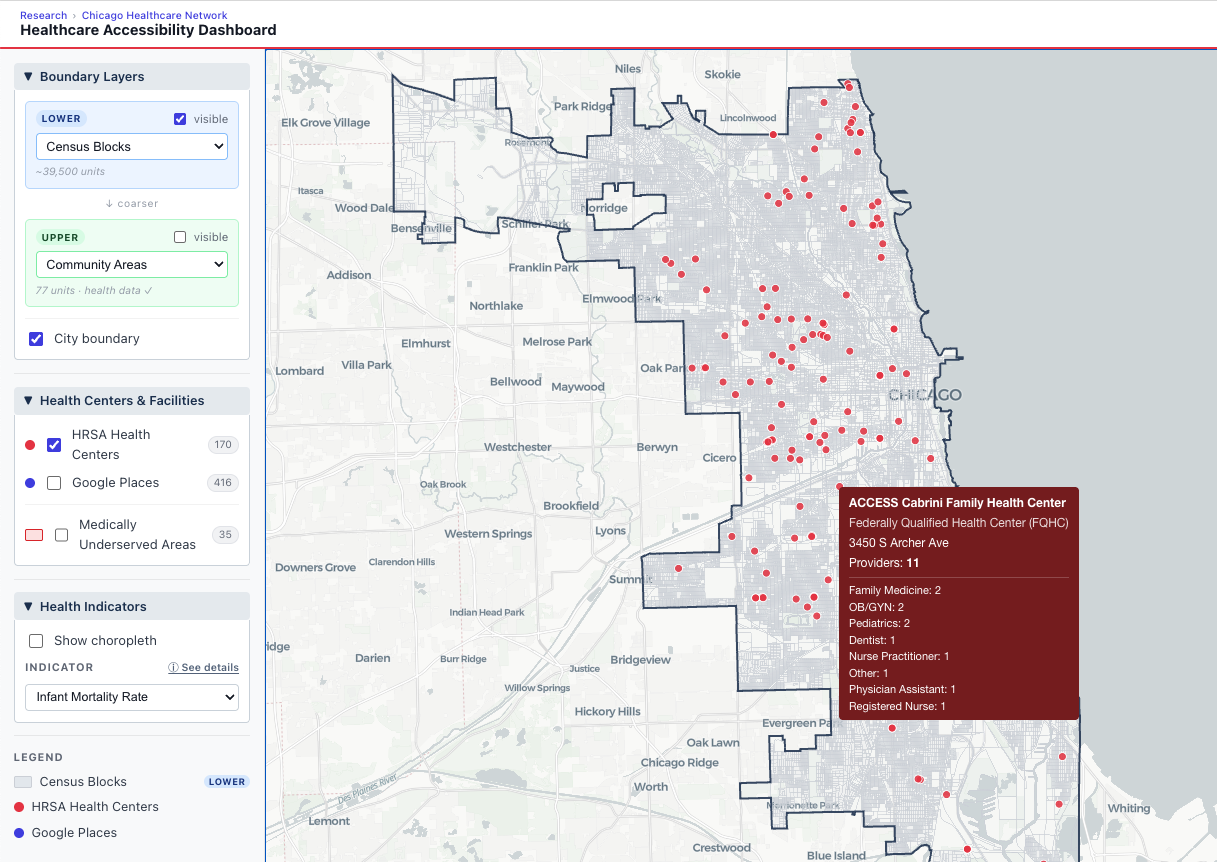
\includegraphics[width=0.75\textwidth]{dashboard.png}
\caption{FQHC sites overlaid on community area boundaries, with infant mortality rate as the tract-level indicator. The tooltip for ACCESS Gabriel Family Health Center illustrates per-site information available on hover: site type, provider count, specialties, and registered services.}
\end{figure}

\begin{figure}[H]
\centering
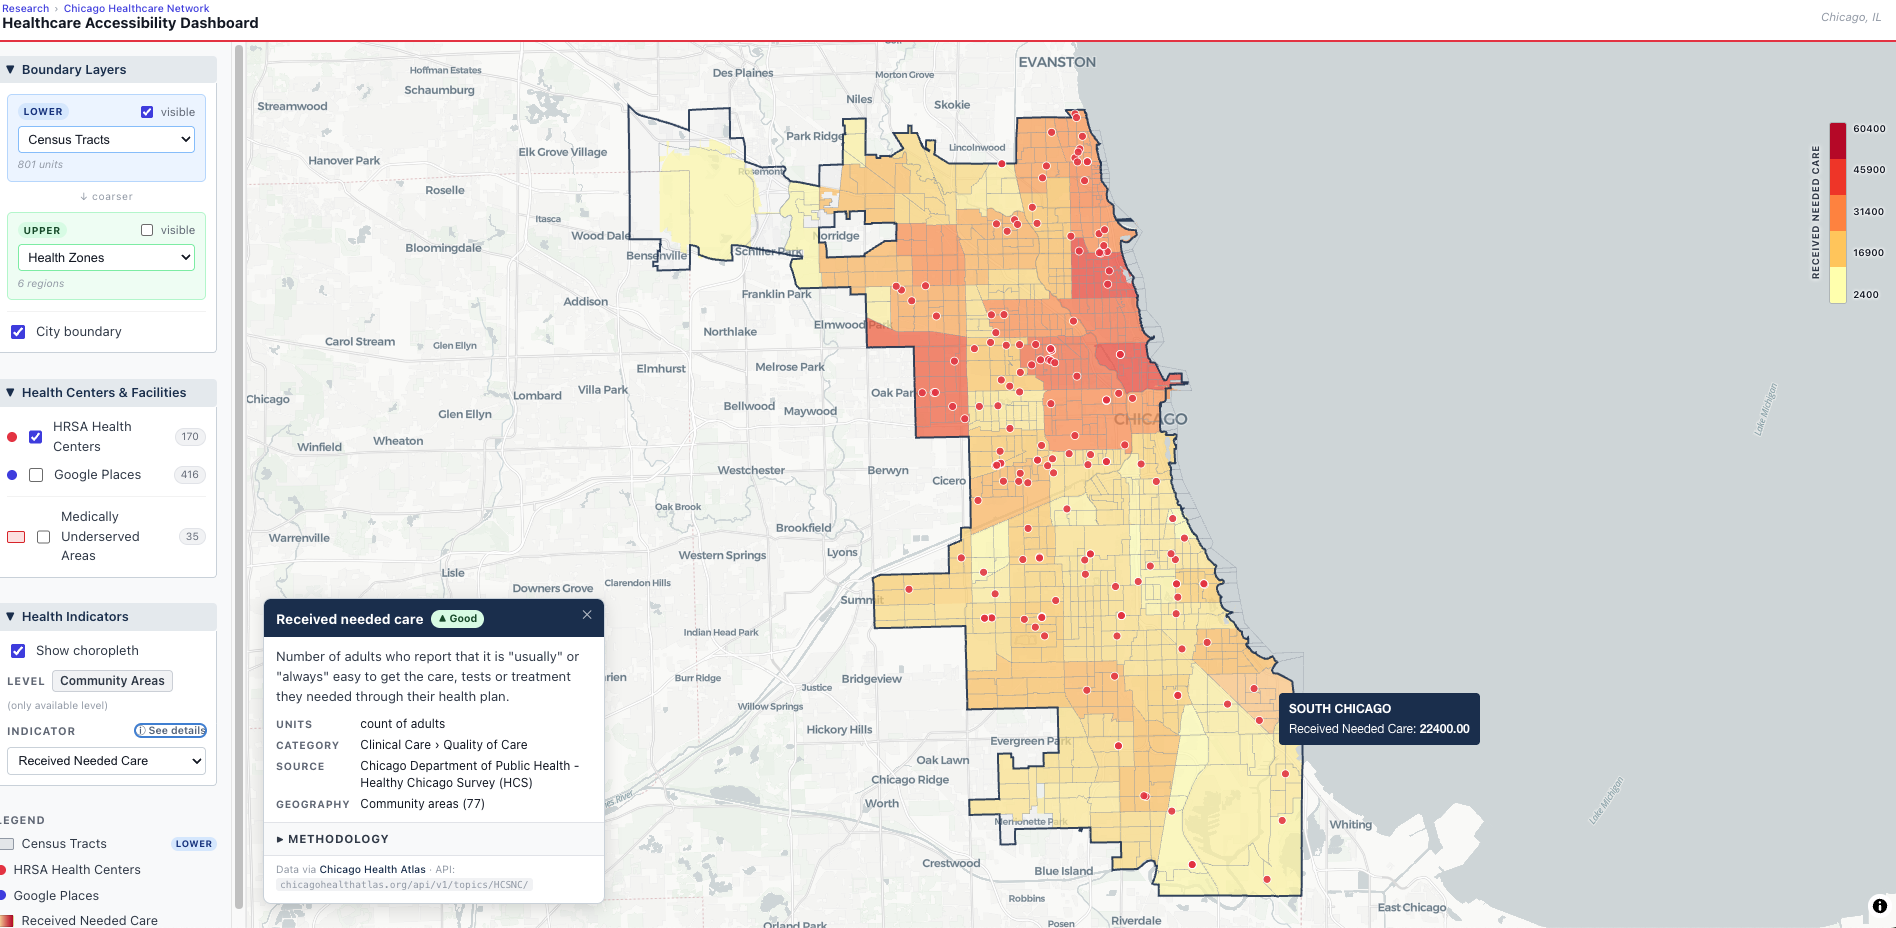
\includegraphics[width=0.75\textwidth]{dashboard3.png}
\caption{Health indicator overlay (``Received Needed Care'' rate) at the census tract level, with FQHC sites and a community area tooltip for South Chicago showing local statistics.}
\end{figure}

\clearpage

\begin{figure}[H]
\centering
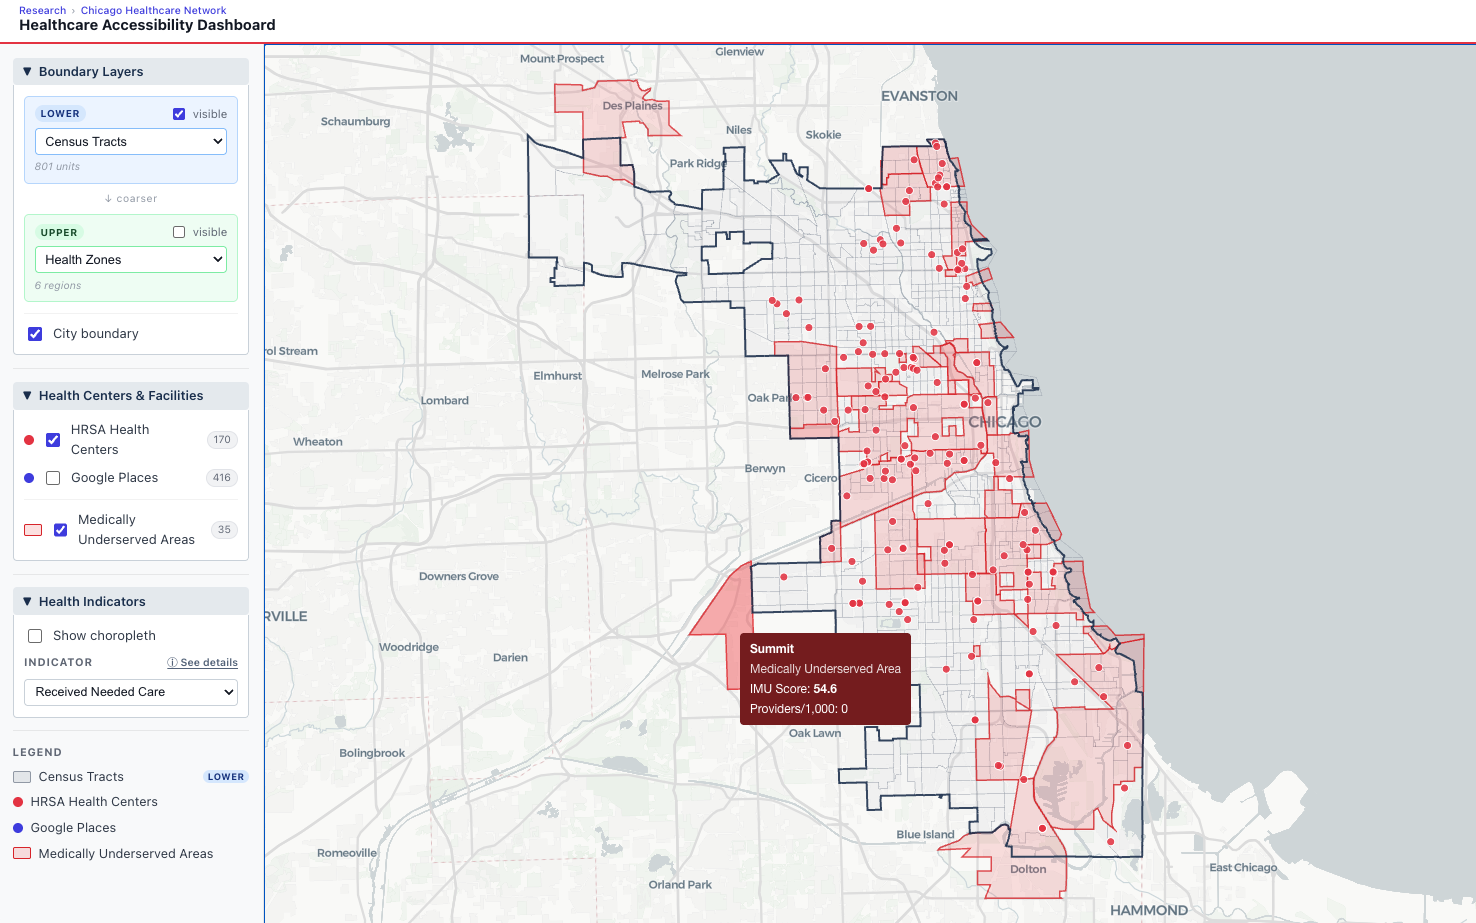
\includegraphics[width=0.75\textwidth]{dashboard2.png}
\caption{All facility layers (FQHCs, hospitals, private clinics) with Health Zone boundaries. The MUA tooltip illustrates per-area information: IMU score and provider counts within that medically underserved area.}
\end{figure}

\begin{figure}[H]
\centering
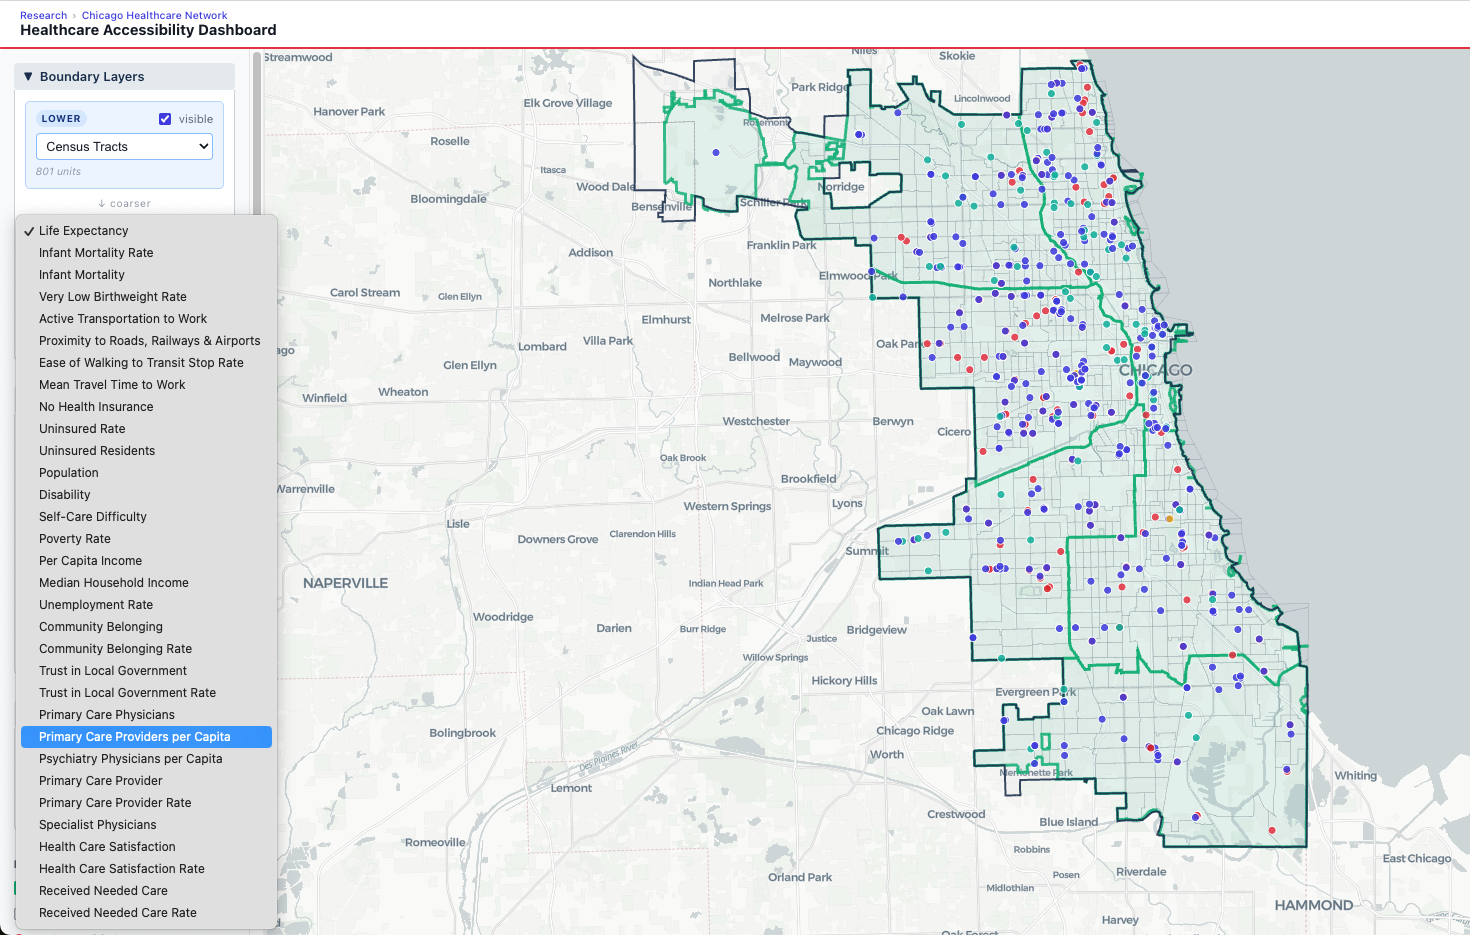
\includegraphics[width=0.75\textwidth]{dashboard4.png}
\caption{The full menu of 33 health indicators available for overlay, including life expectancy, infant mortality, insurance rates, chronic disease prevalence, and primary care provider rates.}
\end{figure}



\end{document}
